%!TEX program = xelatex
%!TEX TS-program = xelatex
%!TEX encoding = UTF-8 Unicode

\documentclass[a4paper]{article}
\usepackage[UTF8, heading = false, scheme = plain]{ctex}
\usepackage{graphicx}
\usepackage{cite}
\usepackage{geometry}
\geometry{left=2.0cm, right=2.0cm, top=2.5cm, bottom=2.5cm}
\usepackage[colorlinks,linkcolor=red,anchorcolor=blue,citecolor=green]{hyperref}
\usepackage{subfig}
\usepackage{caption}
\captionsetup{font={scriptsize}}

\renewcommand\figurename{图}

\makeatletter
\let\@afterindentfalse\@afterindenttrue
\@afterindenttrue
\makeatother
\setlength{\parindent}{2em}  

\linespread{1.4}
\setlength{\parskip}{0.5\baselineskip}
\usepackage{bm}
\title{学习汇报\\第七周}
\author{熊凯亚}
\date{\today}

\begin{document}
\maketitle

本周主要看的是ICLR'17的best paper之一:Semi-supervised knowledge transfer for deep learning from private training data
\paragraph{回顾}

上周主要看了最初提出协作深度学习的文章\cite{shokri2015privacy},了解了一下关于协作深度学习的工作原理。
典型的多层网络中:\\
1.每个神经元会接收到上层神经元的输出加上来自一个特殊神经元的偏移信号,然后根据它的输入计算加权平均值,称为总输入。通过总输入值应用非线性激活函数来计算神经元的输出。\\
2.$K$层的神经网络输出向量为$\bm{a}_k=f(W_k\bm{a}_{k-1})$,其中$f$为激活函数,$W_k$为权重矩阵,它决定了每个输入信号的权重。
常用的激活函数有如下几个:
\begin{itemize}
\item 双曲正切 $f(z)=(e^{2z}-1)(e^{2z}+1)^{-1}$
\item Sigmoid $f(z)=(1+e^{-z})^{-1}$
\item Rectifier $f(z)=max(0,z)$
\item Softplus $f(z)=log(1+e^z)$
\end{itemize}
3.最后一层的激活函数通常是Softmax函数$f(z_j)=e^{z_j}(\Sigma_ke^{z_k})^{-1},\forall j$ \\
4.最后一层中,每个神经元$j$的输出就是输入属于类$j$的概率。\\
5.越高层计算出的值表示数据的特征越抽象。\\
6.若神经网络用于分类,抽象特征也代表输入输出的关系。\\
7.深度学习的主要挑战是从训练数据中自动学习使神经网络的目标(例如分类的准确性)最大化的参数值(权重矩阵)。\\
8.梯度下降始于随机点(由神经网络的参数决定),然后每步计算被优化的非线性函数的梯度并更新参数以减少梯度。一直持续到算法收敛到局部最优。\\
9.每个权重参数的梯度由feed-forward前向反馈和back-prapagation后向传播过程计算出来。

\section{PATE}

本周看了Google在ICLR'17上发表的文章\cite{Papernot2016SemisupervisedKT}用半监督知识迁移解决深度学习中训练数据隐私问题,为了解决这个问题这篇文章提出了PATE(Private Aggregation of Teacher Ensembles)教师全体的隐私聚合的概念。

\begin{enumerate}
\item Model Inversion Attacks 通过机器学习模型的预测结果,可以反过来重建模型训练时使用的数据。
\item Membership Inference Attacks 可以根据模型的预测结果,来推理出模型训练数据中是否包含了某个具体的训练点(training point)。
\end{enumerate}
对机器(深度)学习模型的攻击:
\begin{enumerate}
\item model querying 攻击者通过查询来观察模型。对于攻击者而言模型是一个黑盒,攻击者可以挑选输入值来观察模型的预测结果。
\item model inspection 属于白盒攻击。例如上次看的一篇论文Deep model under the GAN中提到的协作学习中的参与者对模型进行的白盒攻击。
\end{enumerate}
威胁模型:
\begin{itemize}
\item 攻击者可以进行潜在的无限多的查询。
\item 攻击者能够进入模型内部组件。
\end{itemize}

\subsection*{教师模型}

首先,将待训练的敏感数据分为互斥的$N$份不同数据集,然后由这些数据集分别独立训练不同的模型,得到$N$个教师模型。当部署训练好的教师模型时,需要记录每一个教师模型对于查询的预测结果,选取票数最高的那个,并将预测结果聚合起来。如果大部分教师模型都同意某一个预测结果,那就意味着它不依赖于具体的分散数据集,所以隐私成本很小。但是,如果有两类预测结果有相近的票数,那么这种不一致,或许会泄露隐私信息。

因此,在中间统计最高票数之后引入拉普拉斯噪声,将票数的统计情况打乱,从而保护了隐私。教师模型的训练及聚集过程如图\ref*{fig:overview}左侧部分所示。

\begin{figure}[!h]
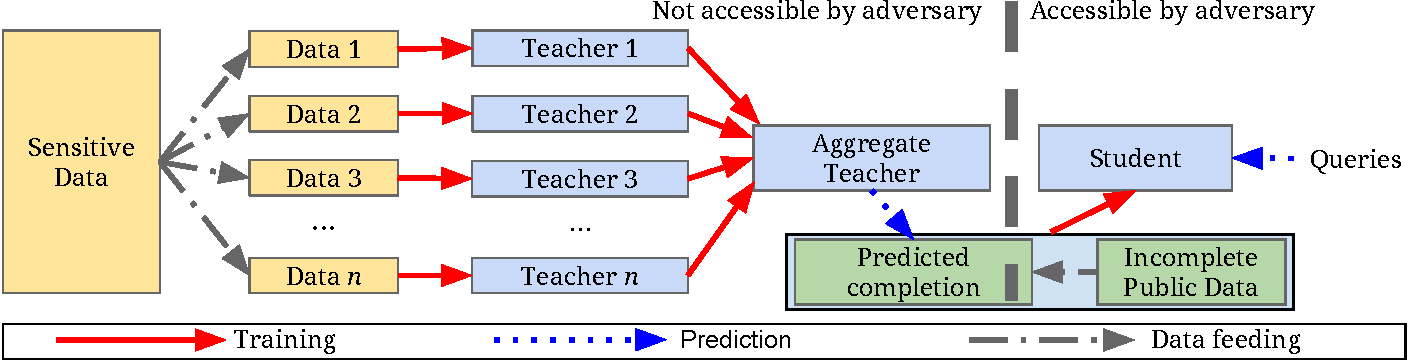
\includegraphics[width = \linewidth]{fig/approach-overview.pdf}
\caption{教师模型的聚集过程(左侧部分)和学生模型(右侧部分)}
\label{fig:overview}
\end{figure}

\subsection*{学生模型}

聚合教师模型(Aggregated Teacher)可以看作是一个差分隐私API,用户提交输入值,他就会返回相应的标签,同时又能保护隐私。但是,如果能训练一个机器学习模型,部署到用户设备上直接运行模型得出预测结果,这样的话肯定会更好。因此,又训练了一个额外模型:学生模型。学生模型可以获得未标记的公共数据集。为了训练学生模型,需要聚合教师模型以隐私保护的方式,来给公共数据进行标注,传递知识。用于部署在设备上的,就是训练好的学生模型。
\subsection*{学生模型的必要性}

实际上聚合教师模型破坏了之前所说的威胁模型,每次在查询聚合教师模型时,都会增加隐私成本,因为它每次给出的输出结果都会或多或少地透露出一些隐私信息。然而,当学生模型训练好之后,只能对聚合教师模型进行固定数量的查询,那么隐私成本就会被固定下来了。

另外,还需要防范攻击者探取模型底层函数库。教师模型是由隐私数据训练的,学生模型是由公共数据(非隐私数据)训练的,带有隐私保护的标注。所以最坏的情况是,攻击者通过查验学生模型的底层函数库而获得其训练数据,即使这样攻击者也只能得到带有隐私保护的标注信息,除此以外攻击者得不到再多的隐私信息了。

\subsection*{PATE-G}

PATE-G是PATE的一种生成式变种,它使用对抗生成网络GAN来减少训练学生模型时所需的标签数目。PATE-G的设计初衷很简单:我们希望产生学生模型训练时需要用的标签数目,数目越小,则隐私成本越小。

生成对抗网络(GANs)的一般架构是分为生成器和判别器。我们将原本二元分类的判别器(只判别数据是真实的 or 生成的)扩展至一个多类别的分类器,用来区分:已标注的真实样本,未标注真实样本,以及生成样本\cite{Salimans2016ImprovedTF}。

\section{实验}

本实验主要在MNIST和SVHN数据集上训练。图\ref{fig:teacher-accuracy}描绘了聚合教师模型的准确率。所以,在训练学生模型之前,需要考虑了每一个标签的隐私。横轴是每一个标签查询的$\epsilon$值,纵轴是预测结果的平均准确率。
\begin{figure}
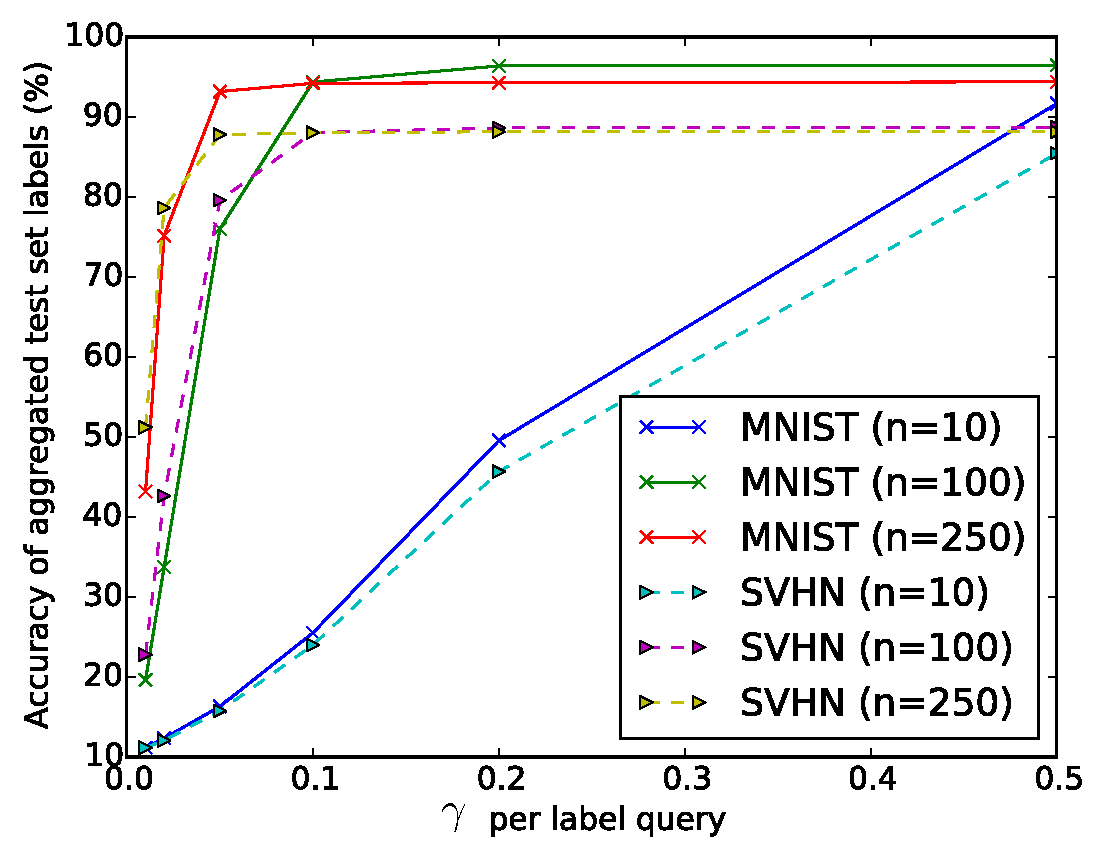
\includegraphics[width = 3in]{fig/lap-scale-accuracy.pdf}
\caption{聚合教师准确率}
\label{fig:teacher-accuracy}
\end{figure}
紫色的线代表了一个包含10个教师模型的聚合教师模型($n=10$)。当逐渐降低$\epsilon$的值,意味着我们引入更多的随机噪声,加强隐私保护,那么这个聚合教师模型的准确率也很快下降。但是,图中绿线和红线的部分,分别是包含100个和250个教师模型的聚合教师模型($n=100, n=250$),那么在较低$\epsilon$值时,仍然可以保持较高的准确率。

\section{总结}
\begin{enumerate}
\item 第一点,就是这个方法是具有通用性的,这意味着可以将它应用于各种分类器中(包括神经网络)。
\item 第二点,差分隐私范围(bound)不是给定的,对于达到准确度与隐私之间的良好的平衡,具有重要意义。
\item 第三点,隐私和通用性并不一定是互相矛盾的。
\end{enumerate}

\section{想法}
在协作深度学习中,Hitaj等人通过在恶意参与者方训练GAN模型获得受害参与者的训练数据\cite{hitaj2017deep},这一攻击过程属于白盒攻击。本文提出的PATE可以防范一些针对学习模型(trained model)的黑盒攻击。是否可以将PATE与协作深度学习结合起来考虑呢(正在考虑可行性)。

\bibliographystyle{IEEEtran}
\bibliography{references}
\end{document}


